\scanpage{3}
\diagram{\begin{tikzcd}[row sep=small]
\text{disques découpés avec origine fixée}\arrow[d,leftrightarrow]\\
\text{\deleted{\unsure{gr.}} arbre circularisé pointé}
\end{tikzcd}}

\deleted{\unsure{mots}} type de mots \deleted{\unsure{en}} $=$ \deleted{\unsure{disq}} arbres \inserted{plans ou} pointés, \deleted{\unsure{et coupés}} bouts libres, \uline{en l'origine} seult et \deleted{\unsure{orientés}} \inserted{\deleted{\illegible{1}}} \unsure{plats|plat} à l'origine

\diagram{\begin{tikzcd}[column sep=small]
\begin{gathered}\text{disques \inserted{or.} découpés}\\\text{par cordes}\end{gathered}\arrow[r,leftrightarrow]&
\text{\deleted{graphes}\inserted{arbres} circularisés}\arrow[r,leftrightarrow]&
\begin{gathered}\text{contours}\\\text{à involuti.}\\\text{ss pt fixe}\\\text{non \unsure{pénétrante|pointés}}\end{gathered}
\end{tikzcd}}
\diagram{\begin{tikzcd}[column sep=small]
\begin{gathered}\text{disques \inserted{or.}}\\\text{\deleted{\unsure{polygones|topologiquement}}}\\\text{découpés,}\end{gathered}\arrow[r,leftrightarrow]&
\begin{gathered}\text{\deleted{graphes}\inserted{arbres}}\\\text{(à bouts libres)}\\\text{circularisés}\end{gathered}\arrow[r,leftrightarrow]&
\begin{gathered}\text{contours}\\\text{à inv.}\\\text{\unsure{cpt.} \unsure{lin.}}\\\text{\unsure{ss} pt fixe}\\\text{non}\\\text{\unsure{pénétrante|pointés}}\end{gathered}
\end{tikzcd}}
avec condition que chaque cpt. découpée contient \deleted{\unsure{au}} moins un sommet, ou au plus un sommet (au choix)

\figure{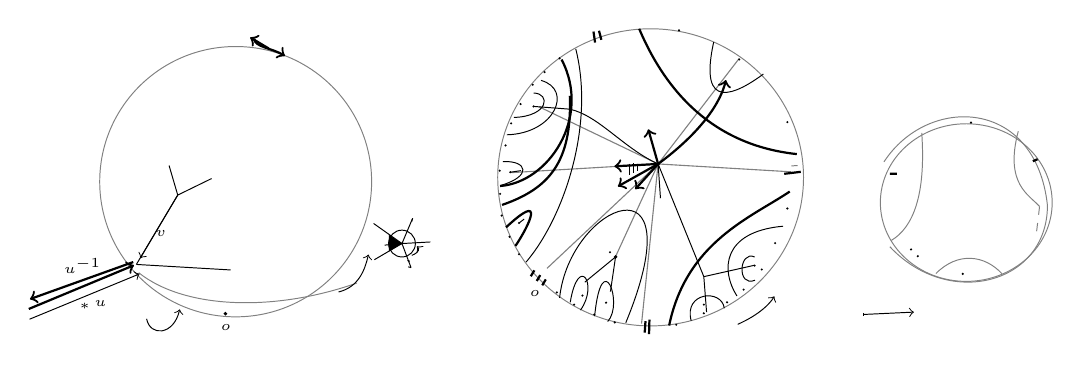
\begin{tikzpicture}[x=.005cm,y=-.005cm,every node/.style={font=\tiny,inner sep=1pt},line width=.35pt]
\draw[gray] (670,640) ellipse(345 and 343);
\draw[gray] (424,871)..controls(542,965)and(772,970)..(978,897);\draw[->,thick] (717,277)..controls(718,299)and(763,301)..(795,321);\draw[->,thick] (754,302)--(707,274);
\draw (418,850)--(523,674)--(501,599) (523,674)--(609,632) (418,850)--(657,864);\draw[->] (523,674)--(428,834);
\draw[->,thick] (410,844)--(148,938);\draw[->,thick] (145,963)--(412,852);\draw[->] (147,989)--(426,874);
\node at (282,853) {$u^{-1}$};\node at (327,950) {$u$};\node at (287,955) {$*$};\node at (480,771) {$v$};
\fill (644,975) circle(5);\node at (645,1011) {$o$};\draw[->] (444,988)..controls(453,1034)and(513,1030)..(528,964);
\draw (1092,797) circle(34);\draw (1092,797)--(1020,746) (1092,797)--(1119,733) (1092,797)--(1164,793) (1092,797)--(1115,858) (1092,797)--(1022,838);\fill (1092,797)--(1059,775)--(1059,817)--cycle;\draw[->] (1117,827)..controls(1139,818)and(1135,809)..(1130,804);\draw[->] (931,920)..controls(983,907)and(998,863)..(1007,825);
\draw (1092,797)--(1048,801) (1119,733)--(1117,741) (1112,842)--(1106,840) (1115,858)--(1108,856);
\draw[gray] (1723,629) ellipse(388 and 377);
\draw[gray,thin] (1742,595)--(1440,450) (1742,595)--(1370,617) (1742,595)--(1460,860) (1742,595)--(1635,828) (1742,595)--(1700,1000) (1742,595)--(2080,615) (1742,595)--(1948,327); \foreach \x/\y in {1345/726,1341/671,1340/612,1355/548,1369/492,1393/443,1424/394,1454/362,1492/327,1795/256,1948/330,2070/489,2070/708,2039/796,2005/863,1959/914,1917/946,1788/1003,1632/997,1580/977,1529/952,1485/921,1437/887,1389/824,1365/780}{\fill (\x,\y) circle(3);} \draw[thick] (1578,259)--(1582,287) (1592,257)--(1598,280) (2062,620)--(2104,615) (1710,994)--(1708,1023) (1720,990)--(1719,1027) (1428,865)--(1419,880) (1443,877)--(1434,892) (1457,888)--(1448,903); \draw[gray] (2080,600)--(2096,599); \node at (1429,925) {$o$}; \draw (1426,415)..controls(1470,416)and(1465,474)..(1376,477); \draw (1445,383)..controls(1527,406)and(1480,518)..(1358,521); \draw[thick] (1497,330)..controls(1574,477)and(1464,642)..(1341,651); \draw (1533,303)..controls(1582,497)and(1503,731)..(1407,844); \draw[thick] (1518,422)..controls(1524,592)and(1464,658)..(1346,699); \draw (1348,589)..controls(1410,586)and(1424,626)..(1341,650); \draw (1367,616)--(1394,612) (1389,745)--(1402,735); \draw[thick] (1356,756)..controls(1458,661)and(1415,751)..(1380,803); \draw (1426,449)--(1518,456)..controls(1591,472)and(1654,555)..(1742,595); \draw[thick] (1694,252)..controls(1760,408)and(1879,547)..(2094,570); \draw[thick,->] (1742,595)..controls(1853,513)and(1901,438)..(1914,382); \draw (1883,286)..controls(1843,467)and(1941,417)..(2009,367); \draw (1742,595)--(1858,881)--(1865,971) (1858,881)--(1987,852); \draw[thick] (1770,1005)..controls(1814,792)and(1980,730)..(2076,665); \draw (1660,998)..controls(1840,560)and(1517,697)..(1492,935); \draw (1519,946)..controls(1540,821)and(1592,900)..(1545,966); \draw (1581,981)..controls(1599,798)and(1656,950)..(1614,995); \fill (1634,831) circle(5);\draw (1634,831)--(1621,919) (1634,831)--(1556,895); \draw (1826,993)..controls(1806,920)and(1903,911)..(1910,961); \draw (2059,753)..controls(1903,767)and(1901,866)..(1942,930); \draw (1987,831)..controls(1947,813)and(1941,910)..(1988,890); \draw[->] (1944,1002)..controls(2000,977)and(2026,949)..(2037,931); \foreach \x/\y in {1426/449,1367/616,1389/745,1620/819,1858/952,1858/974,1987/853}{\fill (\x,\y) circle(3);} \draw[thick,->] (1742,595)--(1717,507);\draw[thick,->] (1742,595)--(1631,601);\draw[thick,->] (1742,595)--(1640,652);\draw[thick,->] (1742,595)--(1684,659);\draw (1742,595)--(1748,682);\fill (1742,595) circle(5);\draw (1670,594)--(1670,622) (1680,593)--(1680,618) (1690,594)--(1690,614); \fill (1550,929) circle(3) (1610,947) circle(3);
\draw[gray] (2524,693) ellipse(218 and 200);\draw[gray] (2315,590)..controls(2425,420)and(2700,425)..(2730,700)..controls(2730,900)and(2480,965)..(2330,805) (2411,516)..controls(2422,674)and(2389,756)..(2334,789) (2656,512)..controls(2620,647)and(2685,674)..(2710,703) (2447,873)..controls(2503,817)and(2571,826)..(2615,874); \foreach \x/\y in {2536/490,2384/812,2401/829,2515/874}{\fill (\x,\y) circle(3);}\draw[gray,dashed] (2710,703)--(2701,779); \draw[->] (2262,977)--(2391,971);\draw (2263,973)--(2263,980); \draw[thick] (2330,620)--(2348,620) (2693,588)--(2705,583);
\end{tikzpicture}}

\par\noindent\uline{NB} Alors l'ens. des arêtes issues d'un sommet quelq. est canoniq$^{t}$ \uline{ordonné}\par

\figure{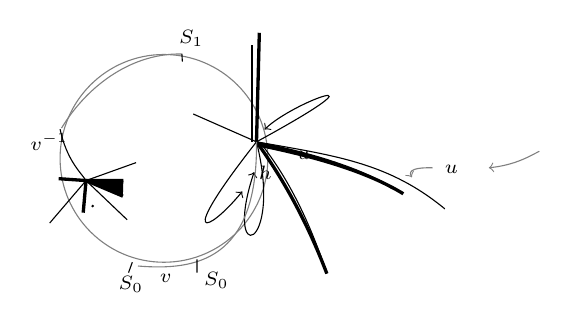
\begin{tikzpicture}[x=.006cm,y=-.006cm,every node/.style={font=\scriptsize,inner sep=1pt}]
\draw[gray] (365,350) ellipse(220 and 220);
\draw[gray] (148,286)..controls(205,192)and(301,126)..(404,129);
\draw (145,288)..controls(159,354)and(189,380)..(200,397);
\fill (200,397) circle(4) (561,315) circle(4);
\fill (200,397)--(279,397)--(278,430)--cycle;
\draw[very thick] (200,397)--(142,393) (200,397)--(279,397) (200,397)--(278,430) (200,397)--(194,465);
\draw (200,397)--(306,359) (200,397)--(287,480) (200,397)--(123,487);\fill (214,451) circle(3);
\draw (561,315)--(427,256);
\draw[very thick] (561,315)--(567,84);
\draw[thick] (551,315)--(551,110);
\draw (561,315)..controls(733,345)and(842,360)..(960,457);
\draw[very thick] (566,322)..controls(680,345)and(794,377)..(872,425);
\draw[thick] (565,317)..controls(680,340)and(785,373)..(850,414);
\draw[very thick] (561,315)..controls(624,402)and(672,495)..(710,594);
\draw (570,318)..controls(637,403)and(680,503)..(710,594);
\draw[->] (561,315)..controls(862,151)and(639,229)..(578,289);
\draw[->] (561,315)..controls(387,536)and(457,510)..(531,420);
\draw[->] (561,315)..controls(619,548)and(488,582)..(556,379);
\draw[gray] (561,315)..controls(564,567)and(432,588)..(310,578);
\draw (403,129)--(404,145) (298,570)--(290,592) (435,564)--(435,592);
\node at (423,96) {$S_1$};\node at (122,315) {$v^{-1}$};\node at (295,617) {$S_0$};\node at (369,604) {$v$};\node at (476,608) {$S_0$};\node at (661,343) {$u$};\node at (580,380) {$h$};\node at (974,374) {$\unsure{u}$};\draw[gray,->] (934,370)..controls(900,369)and(881,374)..(890,390);
\draw[gray,<-] (1053,370)..controls(1110,364)and(1140,345)..(1160,335);
\end{tikzpicture}}

La cat. des ``\deleted{\unsure{mots}}\inserted{types} de mots'' de long. $n$ \unsure{équivaut|équiv.-t} \unsure{à|:} la cat. \unsure{isotypique|isotopique} des systèmes formés d'un disque $D$ \inserted{en général orienté} d'un ``découpage par cordes'' de ce disque, avec au moins un sommet sur chaque arête découpée sur $\dot D$ par les extrémités des cordes,
\[
(D,\omega,\deleted{\unsure{K|S_0}},\deleted{\unsure{S}},K,S_0)
\]
$D$ le disque top.\par
$\omega$ une orientation de $D$\par
$K\subset D$ le 1-complexe top. (\unsure{réunion} top. de segments) des cordes du découpage\par
$S_0\in S$ \deleted{\unsure{est la composante} \unsure{de} \unsure{$\pi_0$|l'origine} $(\dot D\unsure{\setminus}K\cap\dot D)$}\par
\noindent\begin{tabular}{@{}ll@{}}
$S\subset\dot D$, & soit $R_0$ l'unique comp. connexe de\\
\unsure{et|de} $S\ne\varnothing$ & $D\setminus K$ contenant $S_0$
\end{tabular}

\[
\uline{\text{ordre réduit}}=\sum_{\alpha\in\pi_0(\dot D\setminus K\cap\dot D)}(\operatorname{Card}(\alpha\cap S)-1)
\]
\[
(\deleted{\text{\unsure{pour|ou}}\ \unsure{\alpha\in\pi_0}}\ \alpha\subset R_0)
\]
\margin{$v\,u^{-1}u$\par $u\,v\cdot u^{-1}$}

\noindent\begin{minipage}[t]{.39\linewidth}
Type de mot \uline{trivial} : ordre réduit $=0$\par
\uline{Type de mot totalitaire} : $K=\varnothing$\par
(\unsure{non|i.e.} trivial)
\end{minipage}\hfill\begin{minipage}[t]{.02\linewidth}\figure{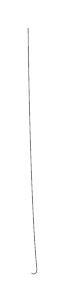
\begin{tikzpicture}[x=.014cm,y=-.014cm]\draw[gray,line width=.3pt] (1124,1921) .. controls (1125,2010) and (1128,2100) .. (1132,2140) .. controls (1132,2144) and (1129,2145) .. (1127,2143);\end{tikzpicture}}\end{minipage}\hfill\begin{minipage}[t]{.56\linewidth}
\[
\operatorname{Card}S=n\quad(\ne0)\qquad\text{donc }S\ne\varnothing
\]
\[
\deleted{\unsure{S\cap S_0\ne\varnothing}}\quad
\forall\alpha\in\pi_0(\dot D\setminus K\cap\dot D)
\left\{\begin{array}{l}
S\cap\alpha\ne\varnothing\\
\operatorname{Card}S\cap\alpha=1\quad\text{si }\alpha\not\subset R_0
\end{array}\right.
\]
Type de mot trivial,\par
si $\unsure{2}\ \operatorname{Card}S\cap\alpha$
\end{minipage}

\par\noindent{\ttfamily
/*JOB=CRAY1,ACCT=*********,ALL=\unsure{M06|MO6}\\
// JOB MSGLEVEL=(1,1),MSGCLASS=A\\
// EXEC CSSBATCH\\
//CRAYIN DD *\par}
\par\noindent{\ttfamily\unsure{J0202CNU|JO202CNU}}\par
\margin{2}
